\begin{frame}{Phase retrieval}
    \begin{columns}

        \column[T]{0.58\textwidth}
        \begin{figure}
            \centering
            \animategraphics[width=\textwidth,autoplay,loop]{1}{Figures/gwaihir/animated_pr/merged_image_}{1}{10}
            \caption{Phase retrieval with PyNX using iterative algorithms. \footnotemark}
            \label{fig:pr_pynx}
        \end{figure}

        Bragg electronic density:
        \begin{equation*}
            \rho_{crystal}(\Vec{r}) \exp^{i(\Vec{q}_{hkl}.\Vec{u}
            (\Vec{r}))}
        \end{equation*}

        \column[T]{0.38\textwidth}
    
        \begin{figure}
            \centering
            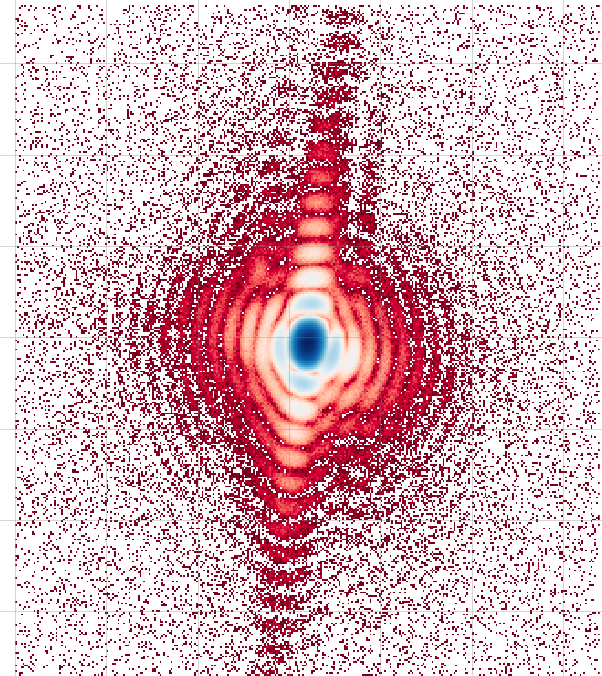
\includegraphics[width=0.8\textwidth]{Figures/gwaihir/dp_pr.png}
            \pause
            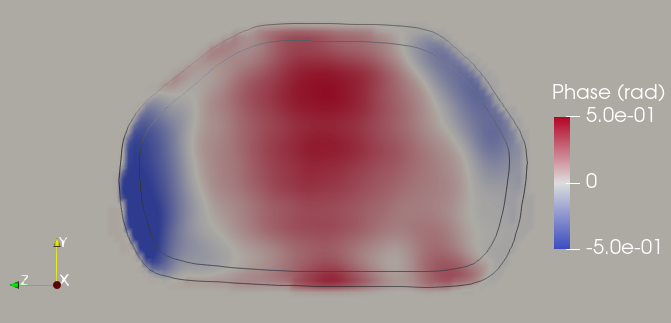
\includegraphics[width=0.8\textwidth]{Figures/gwaihir/obj_pr.png}
            \caption{Bragg peak (top) and reconstructed particle (bottom).}
            \label{fig:pr_dp_particle}
        \end{figure}

    \end{columns}

    \footnotetext{Favre-Nicolin, V., et al  (2011). Journal of Applied Crystallography, 44(3), 635–640.}
\end{frame}


